% ============================================================
% Corrigé et barème de l'évaluation : Séries de Fourier
% Pôle Formation UIMM - CVDL - BTS Industriel - S. JAUBERT
% Compiler d'abord le cours et l'évaluation (fichiers .aux), puis ce corrigé (deux passes).
% ============================================================
\documentclass[a4paper,11pt]{article}
\usepackage[utf8]{inputenc}
\usepackage[T1]{fontenc}
% babel-french absent sur certains postes : chargement conditionnel
\IfFileExists{french.ldf}{\usepackage[french]{babel}}{}
\usepackage{helvet}
\usepackage{courier}
\renewcommand{\familydefault}{\sfdefault}
\usepackage[top=3cm, bottom=2.5cm, left=2cm, right=2cm, headheight=2cm]{geometry}
\usepackage{amsmath,amssymb,amsfonts}
\usepackage{graphicx}
\usepackage[dvipsnames,table]{xcolor}
\usepackage{tikz}
\usepackage{pgfplots}
\pgfplotsset{compat=1.18}
\usepackage[most]{tcolorbox}
\usepackage{fancyhdr}
\usepackage{enumitem}
\usepackage{array,needspace}
\usepackage{titlesec}
\usepackage{xr-hyper}
\usepackage{hyperref}
\externaldocument[C-]{MOD13_Series_Fourier_Cours_v1_0}
\externaldocument[E-]{MOD13_Series_Fourier_Evaluation_v1_0}

\definecolor{uimmblue}{HTML}{005C85}
\definecolor{uimmred}{HTML}{D31326}
\definecolor{uimmlightblue}{HTML}{E8F1F8}
\definecolor{uimmgray}{HTML}{333333}
\definecolor{uimmlightgray}{HTML}{F5F5F5}
\hypersetup{colorlinks=true, linkcolor=uimmblue, urlcolor=uimmblue}

\titleformat{\section}{\Large\bfseries\color{uimmblue}}{}{0pt}{}[\vspace{2pt}{\color{uimmblue}\titlerule[1.2pt]}]
\setlist[enumerate,1]{label={\color{uimmblue}\textbf{\arabic*.}}}
\setlist[enumerate,2]{label=\alph*)}
\setlist[itemize,1]{label={\color{uimmblue}\textbullet}}

\newtcolorbox{correction}[1][]{%
  colback=green!5, colframe=green!50!black,
  fonttitle=\bfseries\color{white}, title={\textsf{Correction}~#1},
  coltitle=white, boxrule=1pt, arc=3pt,
  left=8pt, right=8pt, top=6pt, bottom=6pt, before skip=8pt, after skip=8pt, breakable}
\newtcolorbox{piege}{%
  colback=uimmred!5, colframe=uimmred!80!black, boxrule=1pt, arc=3pt,
  left=8pt, right=8pt, top=5pt, bottom=5pt, before skip=6pt, after skip=6pt}

\newcommand{\M}[1]{\begin{pmatrix}#1\end{pmatrix}}
% Référence vers le cours : §section, page
\newcommand{\cours}[1]{§\ref{C-#1} p.~\pageref{C-#1}}
% Ligne de références en tête de chaque correction
\newcommand{\source}[2]{{\footnotesize\color{uimmgray}\textbf{Réf.} \enspace Énoncé : Évaluation MOD13 p.~\pageref{E-#1} \enspace$\bullet$\enspace Cours MOD13 : #2}\par\smallskip}
\newcommand{\annexe}[1]{annexe p.~\pageref{C-#1}}
\newcommand{\q}[1]{\textbf{\color{uimmblue}#1}\ }

\pagestyle{fancy}
\fancyhf{}
\renewcommand{\headrulewidth}{0pt}
\fancyhead[L]{\raisebox{-0.5\height}{
\includegraphics[height=1.5cm]{logo_uimm_placeholder.jpg}}}
\fancyhead[C]{\begin{minipage}{8cm}\centering
  {\small\color{uimmblue}\textbf{Pôle Formation UIMM - CVDL}}\\
  {\footnotesize\color{uimmgray} BTS Industriel -- Mathématiques}\end{minipage}}
\fancyhead[R]{{\small\color{uimmred}\textbf{MOD13 -- Corrigé Éval}}}
\fancyfoot[C]{{\color{uimmblue}\rule{\textwidth}{1pt}}\\[2pt]
  {\footnotesize\color{uimmgray} Pôle Formation UIMM -- Centre-Val de Loire \hfill S. JAUBERT \hfill \thepage}}

\newcommand{\pts}[1]{\hfill{\color{white}\small\textbf{#1}}}
\newcommand{\bareme}[1]{\par\smallskip{\footnotesize\color{uimmred}\textbf{Barème :} #1}}
\begin{document}

\begin{tcolorbox}[colback=uimmred, colframe=uimmred, sharp corners, boxrule=0pt,
  left=14pt, right=14pt, top=10pt, bottom=10pt]
{\color{white}\LARGE\bfseries Corrigé et barème -- Évaluation MOD13}\\[4pt]
{\color{white}\large Séries de Fourier \hfill Total : 20 points}
\end{tcolorbox}

\begin{tcolorbox}[colback=uimmlightgray, colframe=uimmgray, boxrule=0.8pt, arc=3pt]
\small\textbf{Principes de notation.} Les points de méthode (période et $\omega$ corrects, facteur $\frac2T$, simplification par $(-1)^n$, carrés dans Parseval) sont accordés même en cas d'erreur de calcul. Une erreur n'est sanctionnée qu'une fois : la suite, cohérente avec le résultat faux, est notée normalement. Une conclusion sans unité perd au plus $0{,}25$\,pt par question.
\end{tcolorbox}

\needspace{5cm}
\section{Exercice 1 -- Séries numériques (5 points)}

\begin{correction}[-- Question 1 \pts{1 pt}]
\source{ev:1}{\cours{th:geometrique}}
Série géométrique de raison $0{,}8$, $|0{,}8|<1$ : elle converge, de somme $\dfrac{1}{1-0{,}8} = 5$.
\bareme{convergence justifiée : 0,5 \quad somme : 0,5}
\end{correction}

\begin{correction}[-- Question 2 \pts{1 pt}]
\source{ev:1}{\cours{th:geometrique}}
Premier terme $3\times 0{,}5 = 1{,}5$, raison $0{,}5$ : converge, somme $\dfrac{1{,}5}{1-0{,}5} = 3$.
\bareme{0 point pour $\frac{3}{1-0{,}5} = 6$ (premier terme mal identifié), 0,5 si la convergence seule est justifiée}
\end{correction}

\begin{correction}[-- Question 3 \pts{1 pt}]
\source{ev:1}{\cours{th:riemann}}
Séries de Riemann : $\alpha = 0{,}9\leq 1$, la première diverge ; $\alpha = 2{,}5 > 1$, la seconde converge.
\bareme{0,5 par série}
\end{correction}

\begin{correction}[-- Question 4 \pts{2 pts}]
\source{ev:1}{\cours{ex:graisse}}
Les fuites successives forment une suite géométrique de premier terme $0{,}5$ et de raison $0{,}9$. Volume total : $V = \displaystyle\sum_{n\geq0}0{,}5\times 0{,}9^n = \frac{0{,}5}{1-0{,}9} = 5$\,L.
\bareme{modélisation : 1 \quad convergence : 0,5 \quad résultat avec unité : 0,5}
\end{correction}

\needspace{5cm}
\section{Exercice 2 -- Coefficients d'un créneau (8 points)}

\begin{correction}[-- Question 1 \pts{1 pt}]
\source{ev:2}{\cours{meth:representer} et \cours{subsec:vocabulaire}}
Créneau alternant $10$\,V pendant $10$\,ms et $0$\,V pendant $10$\,ms. $f_0 = \dfrac{1}{0{,}02} = 50$\,Hz ; $\omega = \dfrac{2\pi}{0{,}02} = 100\pi\approx 314$\,rad/s.
\bareme{graphique : 0,5 \quad $f_0$ et $\omega$ : 0,5}
\end{correction}

\begin{correction}[-- Question 2 \pts{1 pt}]
\source{ev:2}{\cours{def:coefficients}}
$a_0 = \dfrac1T\displaystyle\int_0^{T/2}10\,\mathrm dt = \dfrac{10}{T}\times\dfrac T2 = 5$\,V : c'est bien la valeur moyenne lue sur le graphique (le signal passe la moitié du temps à $10$\,V).
\end{correction}

\begin{correction}[-- Question 3 \pts{1,5 pt}]
\source{ev:2}{\cours{meth:coefficients}}
$a_n = \dfrac2T\displaystyle\int_0^{T/2}10\cos(n\omega t)\,\mathrm dt = \dfrac{20}{Tn\omega}\big[\sin(n\omega t)\big]_0^{T/2} = \dfrac{20}{2n\pi}\sin(n\pi) = 0$, car $Tn\omega = 2n\pi$, $n\omega\frac T2 = n\pi$ et $\sin(n\pi) = 0$.
\bareme{intégrale posée avec $\frac2T$ : 0,5 \quad primitive : 0,5 \quad simplification : 0,5}
\end{correction}

\begin{correction}[-- Question 4 \pts{2,5 pts}]
\source{ev:2}{\cours{ex:creneau}}
\[
b_n = \frac2T\int_0^{T/2}10\sin(n\omega t)\,\mathrm dt = \frac{20}{Tn\omega}\big[-\cos(n\omega t)\big]_0^{T/2} = \frac{10}{n\pi}\big(1-\cos(n\pi)\big) = \frac{10}{n\pi}\big(1-(-1)^n\big).
\]
Si $n$ est pair, $1 - 1 = 0$ et $b_n = 0$. Si $n$ est impair, $1 + 1 = 2$ et $b_n = \dfrac{20}{n\pi}$.
\bareme{intégrale : 0,5 \quad primitive et bornes : 1 \quad $\cos(n\pi) = (-1)^n$ : 0,5 \quad deux cas : 0,5}
\end{correction}

\begin{correction}[-- Question 5 \pts{1 pt}]
\source{ev:2}{\cours{def:spectre}}
$A_n = |b_n|$ : $A_1 = \frac{20}{\pi}\approx 6{,}37$\,V ($50$\,Hz) ; $A_2 = 0$ ; $A_3\approx 2{,}12$\,V ($150$\,Hz) ; $A_4 = 0$ ; $A_5\approx 1{,}27$\,V ($250$\,Hz). La composante continue ($5$\,V) figure à $0$\,Hz.
\begin{center}
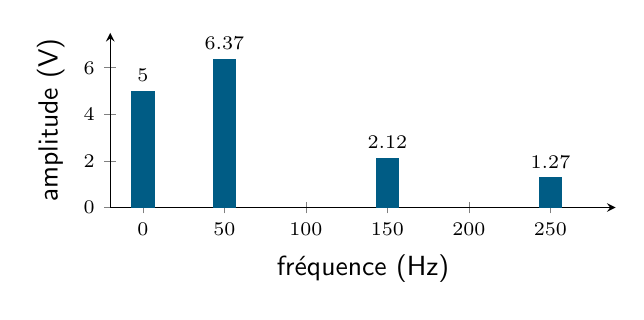
\begin{tikzpicture}
\begin{axis}[width=8cm, height=3.8cm, ybar, bar width=8pt, xlabel={fréquence (Hz)}, ylabel={amplitude (V)},
  ymin=0, ymax=7.5, xmin=-20, xmax=290, xtick={0,50,100,150,200,250}, axis lines=left, nodes near coords,
  every node near coord/.append style={font=\scriptsize}, tick label style={font=\scriptsize}]
  \addplot[fill=uimmblue, draw=uimmblue] coordinates {(0,5)(50,6.37)(150,2.12)(250,1.27)};
\end{axis}
\end{tikzpicture}
\end{center}
\end{correction}

\begin{correction}[-- Question 6 \pts{1 pt}]
\source{ev:2}{\cours{th:parseval} et \cours{ex:parsevalcreneau}}
$\dfrac1T\displaystyle\int_0^T f^2 = \dfrac1T\int_0^{T/2}100\,\mathrm dt = 50$\,V$^2$ (valeur efficace $\sqrt{50}\approx 7{,}07$\,V).\\
$a_0^2 + \frac12b_1^2 = 25 + \frac12\left(\frac{20}{\pi}\right)^2\approx 25 + 20{,}26 = 45{,}26$, soit environ $90{,}5\,\%$ de $50$.
\bareme{valeur exacte : 0,5 \quad part : 0,5 (oublier $a_0^2$ : 0)}
\end{correction}

\needspace{5cm}
\section{Exercice 3 -- Diagnostic vibratoire (7 points)}

\begin{correction}[-- Question 1 \pts{1 pt}]
\source{ev:3}{\cours{ex:lecture}}
$\omega = 50\pi$\,rad/s, donc $f_0 = \frac{50\pi}{2\pi} = 25$\,Hz (fréquence de rotation) et $T = 0{,}04$\,s.
\end{correction}

\begin{correction}[-- Question 2 \pts{1,5 pt}]
\source{ev:3}{\cours{ex:lecture}}
$a_0 = 0$ ; $a_1 = 3$, $b_1 = 4$ ; $a_2 = 0$, $b_2 = 1{,}5$ ; $a_3 = 0{,}5$, $b_3 = 0$.
\bareme{0,5 par harmonique}
\end{correction}

\begin{correction}[-- Question 3 \pts{1,5 pt}]
\source{ev:3}{\cours{def:spectre} et \cours{ex:spectrecapteur}}
$A_1 = \sqrt{3^2 + 4^2} = 5$ ; $A_2 = 1{,}5$ ; $A_3 = 0{,}5$ (en mm/s), à $25$, $50$ et $75$\,Hz.
\begin{center}
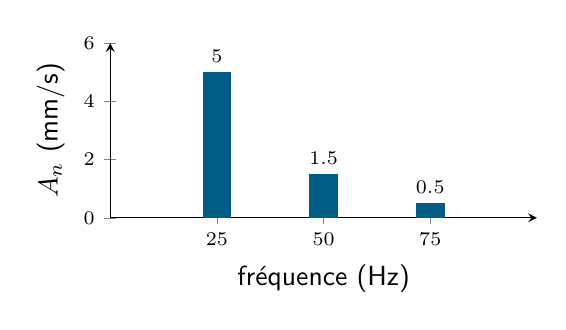
\begin{tikzpicture}
\begin{axis}[width=7cm, height=3.8cm, ybar, bar width=10pt, xlabel={fréquence (Hz)}, ylabel={$A_n$ (mm/s)},
  ymin=0, ymax=6, xmin=0, xmax=100, xtick={25,50,75}, axis lines=left, nodes near coords,
  every node near coord/.append style={font=\scriptsize}, tick label style={font=\scriptsize}]
  \addplot[fill=uimmblue, draw=uimmblue] coordinates {(25,5)(50,1.5)(75,0.5)};
\end{axis}
\end{tikzpicture}
\end{center}
\bareme{$A_1$ : 0,5 \quad $A_2$, $A_3$ : 0,5 \quad spectre : 0,5}
\end{correction}

\begin{correction}[-- Question 4 \pts{1 pt}]
\source{ev:3}{\cours{ex:filrouge}}
La raie 1× ($25$\,Hz) domine nettement : on suspecte un \textbf{balourd}.
\end{correction}

\begin{correction}[-- Question 5 \pts{1,5 pt}]
\source{ev:3}{\cours{ex:niveauglobal}}
$a_0 = 0$ ; par Parseval, $V_{\text{eff}} = \sqrt{\dfrac{A_1^2 + A_2^2 + A_3^2}{2}} = \sqrt{\dfrac{25 + 2{,}25 + 0{,}25}{2}} = \sqrt{13{,}75}\approx 3{,}71$\,mm/s.
\bareme{formule : 0,5 \quad calcul : 0,5 \quad unité : 0,5 ; 0 pour $\sqrt{A_1+A_2+A_3}$ ou $A_1 + A_2 + A_3$}
\end{correction}

\begin{correction}[-- Question 6 \pts{0,5 pt}]
\source{ev:3}{\cours{th:simplification}}
Non : un signal pair n'a que des cosinus ($b_n = 0$), or $b_1 = 4\neq 0$.
\end{correction}

\end{document}
